% Этот шаблон документа разработан в 2014 году
% Данилом Фёдоровых (danil@fedorovykh.ru) 
% для использования в курсе 
% <<Документы и презентации в \LaTeX>>, записанном НИУ ВШЭ
% для Coursera.org: http://coursera.org/course/latex .
% Исходная версия шаблона --- 
% https://www.writelatex.com/coursera/latex/5.3

\documentclass[a4paper,14pt]{article}

% Этот шаблон документа разработан в 2014 году
% Данилом Фёдоровых (danil@fedorovykh.ru) 
% для использования в курсе 
% <<Документы и презентации в \LaTeX>>, записанном НИУ ВШЭ
% для Coursera.org: http://coursera.org/course/latex .
% Исходная версия шаблона --- 
% https://www.writelatex.com/coursera/latex/5.3

% В этом документе преамбула

%%% Работа с русским языком
\usepackage{cmap}					% поиск в PDF
\usepackage{mathtext} 				% русские буквы в формулах
\usepackage[T2A]{fontenc}			% кодировка
\usepackage[utf8]{inputenc}			% кодировка исходного текста
\usepackage[english,russian]{babel}	% локализация и переносы
\usepackage{indentfirst}
\frenchspacing

\renewcommand{\epsilon}{\ensuremath{\varepsilon}}
\renewcommand{\phi}{\ensuremath{\varphi}}
\renewcommand{\kappa}{\ensuremath{\varkappa}}
\renewcommand{\le}{\ensuremath{\leqslant}}
\renewcommand{\leq}{\ensuremath{\leqslant}}
\renewcommand{\ge}{\ensuremath{\geqslant}}
\renewcommand{\geq}{\ensuremath{\geqslant}}
\renewcommand{\emptyset}{\varnothing}

%%% Дополнительная работа с математикой
\usepackage{amsmath,amsfonts,amssymb,amsthm,mathtools} % AMS
\usepackage{icomma} % "Умная" запятая: $0,2$ --- число, $0, 2$ --- перечисление

%% Номера формул
%\mathtoolsset{showonlyrefs=true} % Показывать номера только у тех формул, на которые есть \eqref{} в тексте.
%\usepackage{leqno} % Нумереация формул слева

%% Свои команды
\DeclareMathOperator{\sgn}{\mathop{sgn}}

%% Перенос знаков в формулах (по Львовскому)
\newcommand*{\hm}[1]{#1\nobreak\discretionary{}
{\hbox{$\mathsurround=0pt #1$}}{}}

%%% Работа с картинками
\usepackage{graphicx}  % Для вставки рисунков
\graphicspath{{images/}{images2/}}  % папки с картинками
\setlength\fboxsep{3pt} % Отступ рамки \fbox{} от рисунка
\setlength\fboxrule{1pt} % Толщина линий рамки \fbox{}
\usepackage{wrapfig} % Обтекание рисунков текстом
\usepackage{caption}
\usepackage{subcaption}

%%% Работа с таблицами
\usepackage{array,tabularx,tabulary,booktabs} % Дополнительная работа с таблицами
\usepackage{longtable}  % Длинные таблицы
\usepackage{multirow} % Слияние строк в таблице

%%% Алгоритмы
\usepackage[ruled,vlined]{algorithm2e}

%%% Нумерация уравнений
\usepackage{amsmath}

%%% Теоремы
\theoremstyle{plain} % Это стиль по умолчанию, его можно не переопределять.
\newtheorem{theorem}{Теорема}[section]
\newtheorem{proposition}[theorem]{Утверждение}
 
\theoremstyle{definition} % "Определение"
\newtheorem{definition}[theorem]{Определение}
\newtheorem{heuristics}[theorem]{Эвристика}
\newtheorem{corollary}{Следствие}[theorem]
\newtheorem{problem}{Задача}[section]
 
\theoremstyle{remark} % "Примечание"
\newtheorem*{remark}{Примечание}
\newtheorem*{example}{Пример}
\newtheorem*{nonum}{Решение}

%%% Программирование
\usepackage{etoolbox} % логические операторы

%%% Красивые дроби
\usepackage{nicefrac}

%%% Страница
\usepackage{extsizes} % Возможность сделать 14-й шрифт
\usepackage{geometry} % Простой способ задавать поля
	\geometry{top=20mm}
	\geometry{bottom=20mm}
	\geometry{left=20mm}
	\geometry{right=20mm}
 %
%\usepackage{fancyhdr} % Колонтитулы
% 	\pagestyle{fancy}
 	%\renewcommand{\headrulewidth}{0pt}  % Толщина линейки, отчеркивающей верхний колонтитул
% 	\lfoot{Нижний левый}
% 	\rfoot{Нижний правый}
% 	\rhead{Верхний правый}
% 	\chead{Верхний в центре}
% 	\lhead{Верхний левый}
%	\cfoot{Нижний в центре} % По умолчанию здесь номер страницы

\usepackage{setspace} % Интерлиньяж
\onehalfspacing % Интерлиньяж 1.5
%\doublespacing % Интерлиньяж 2
%\singlespacing % Интерлиньяж 1

\usepackage{lastpage} % Узнать, сколько всего страниц в документе.

\usepackage{soul} % Модификаторы начертания

\usepackage{hyperref}
\usepackage[usenames,dvipsnames,svgnames,table,rgb]{xcolor}
\hypersetup{				% Гиперссылки
    unicode=true,           % русские буквы в раздела PDF
    pdftitle={Заголовок},   % Заголовок
    pdfauthor={Автор},      % Автор
    pdfsubject={Тема},      % Тема
    pdfcreator={Создатель}, % Создатель
    pdfproducer={Производитель}, % Производитель
    pdfkeywords={keyword1} {key2} {key3}, % Ключевые слова
    colorlinks=true,       	% false: ссылки в рамках; true: цветные ссылки
    linkcolor=red,          % внутренние ссылки
    citecolor=black,        % на библиографию
    filecolor=magenta,      % на файлы
    urlcolor=cyan           % на URL
}

\usepackage{csquotes} % Еще инструменты для ссылок

%\usepackage[style=authoryear,maxcitenames=2,backend=biber,sorting=nty]{biblatex}

\usepackage{multicol} % Несколько колонок

\usepackage{tikz} % Работа с графикой
\usepackage{pgfplots}
\usepackage{pgfplotstable}

\author{Бычков Андрей}
\title{Квадратизация дифференциальных уравнений}
\date{\today}

%\includeonly{chapters/Полиномиализация}

\begin{document} 

%\maketitle

\tableofcontents

% !TEX root = ../Диплом.tex

\section{Введение}

Динамические системы являются неотъемлемой частью современной прикладной математики. С помощью динамических систем описываются явления в таких областях как физика \cite{physics-example}, химия \cite{chemistry-example}, биология \cite{biology-example}, экономика \cite{economics-example} и многих других. Математические методы позволяют проводить с ними такие операции как упрощение \cite{MOR-book} и анализировать такие их свойства как устойчивость \cite{Strogatz-book} и достижимость \cite{Scott-reachability}. Многие динамические системы, встречающиеся на практике, описываются с помощью нелинейных дифференциальных уравнений. Анализ таких  систем является молодой областью со множеством открытых вопросов, в отличие от анализа линейных систем \cite{MOR-linear-overview}. Поэтому не удивительно, что многие известные методы для работы с нелинейными системами полагаются на аппрокcимацию нелинейных элементов линейными. К сожалению, такой подход часто ведёт к неудовлетворительным результатам. 
Поэтому большой интерес заслужили подходы, целиком полагающиеся на нелинейную природу систем, которыми они оперируют. 
Отдельно выделим метод понижения порядка моделей QLMOR \cite{Gu-PhD, Kramer-Willcox}, который показывает state-of-the-art результаты, сохраняя при этом динамику исходной системы. 
Данный метод полагается на процесс квадратизации --- приведения систем нелинейных дифференциальных уравнений к системе полиномиальных дифференциальных уравнений степени не более двух. 
Примером квадратизации может послужить следующее преобразование (формальное определение и подробные примеры приведены в главах \ref{sec:definitions}, \ref{sec:polynomialization} и \ref{sec:quadratiaztion}):

\[
     \dot x = \frac{1}{1 + e^x} 
\Longrightarrow
\begin{cases}
    \dot x = y_1 \\
    \dot y_0 = y_0 y_1 \\
    \dot y_1 = -y_1 y_2 \\
    \dot y_2 = y_1 y_2 - 2y_2^2
\end{cases}
\]

На данный момент не существует достаточно эффективных или хотя бы реализованных алгоритмов квадратизации --- она всегда совершается вручную.
Из-за этого, даже для сравнительно небольших систем уравнений проводить её крайне долго и сложно. 
Более того, нет гарантий, что полученная квадратизация имеет наименьшую возможную размерность, что критично в задаче понижения порядка моделей. 

В данной работе мы предлагаем алгоритм квадратизации, описываем его реализацию и модификации, и демонстрируем работу реализации на примерах систем из литературы.
% !TEX root = ../Диплом.tex

\section{Цели и задачи}

Цель данной работы --- предложить и реализовать алгоритм нахождения оптимальной квадратизации систем нелинейных дифференциальных уравнений. Эта задача разбивается на следующие подзадачи:

\begin{enumerate}
    \item Формализовать алгоритм квадратизации.
    \item Предложить алгоритмы поиска оптимальной квадратизации.
    \item Реализовать предложенные алгоритмы внутри системе компьютерной алгебры.
    \item Провести эксперименты, чтобы сравнить работу предложенных алгоритмов.
\end{enumerate}

% !TEX root = ../Диплом.tex

\section{Определения и понятия} \label{sec:definitions}

\subsection{Элементарные нелинейные функции}

\begin{definition}
    Будем понимать под функциями $f_i(\vec x)$ \textit{элементарные нелинейные функции}, которые могут быть записаны как линейные комбинации элементарных функций $g_k(\vec x)$. 
    \begin{equation}
        f_i(\vec x) = p_i^T \vec x + a_{i,1} g_1(\vec x) + \cdots + a_{i,m} g_m(\vec x), p_i \in \mathbb{R}^n, a_j \in \mathbb{R}
    \end{equation}
\end{definition}

Такими функция мы можем покрыть широкий класс проблем, встречающихся на практике. Мы требуем элементарность функций, так как производная элементарной функции может быть найдена за конечное число шагов, что будет критично для нас в дальнейшем.

\subsection{Системы элементарных ОДУ}

В данной работе мы рассматриваем системы нелинейных ОДУ следующего вида:

\begin{enumerate}
    \item \textbf{Система элементарных ОДУ в нормальной форме}
    \begin{equation} \label{eq:ODE-norm-system}
        \begin{array}{cc}
             \dot{x_i} = f_i(\vec x),\quad i = 1 \cdots N
        \end{array}
    \end{equation}
    В теории управления данная форма описывает уравнения состояния для автономных систем.
    
    \item \textbf{Система элементарных уравнений и элементарных ОДУ в нормальной форме}
    \begin{equation} \label{eq:ADE-system}
        \begin{array}{lcl}
             \dot{x_i} = f_i(\vec x), \quad i = 1 \cdots n  \\
             f_j(\vec x) = 0, \quad j = 1 \cdots m
        \end{array},
    \end{equation}
\end{enumerate} 

Как легко заметить, система \eqref{eq:ODE-norm-system} является частным случаем системы \eqref{eq:ADE-system}.



\begin{definition}
    Рассмотрим частный случай систем \eqref{eq:ODE-norm-system} и \eqref{eq:ADE-system}, где функции $f_i$ представляют собой полиномы. Такие системы мы будем называть \textit{полиномиальными}.
\end{definition}

\begin{definition}
    Полиномиальная система имеет порядок $M$, если $M$ - наивысшая степень мономов, образованных переменными $x_i$.
\end{definition}

\begin{definition}
    Полиномиальные системы порядка 2 назовём \textit{квадратичными}.
\end{definition}



% !TEX root = ../Диплом.tex

\section{Полиномиализация} \label{sec:polynomialization}

\begin{definition}
    Процесс преобразования нелинейных систем \eqref{eq:ODE-norm-system}, \eqref{eq:ADE-system} к полиномиальному виду будем называть \textit{полиномиализацией}.
\end{definition}

Далее мы рассмотрим оригинальные алгоритмы квадратизации, описанные в \cite{Gu-PhD}.

\subsection{Полиномиализация с помощью введения алгебраических уравнений} \label{sec:poly-algebraic}

Следующий алгоритм проводит полиномиализацию, добавляя к системе алгебраические уравнения:
\begin{enumerate}
    \item Ввести новую переменную $y_i = g_i(\vec x)$, где $g_i(\vec x)$ - неполиномиальная нелинейная элементарная функция.
    \item Заменить $g_i(\vec x)$ на $y_i$ в оригинальном уравнении.
    \item  Добавить новое уравнение $y_i = g_i(\vec x)$ в систему.
\end{enumerate}

Показанный алгоритм приводит системы вида \eqref{eq:ODE-norm-system}, \eqref{eq:ADE-system} к полиномиальным системам вида \eqref{eq:ADE-system}

\begin{example}
    Рассмотрим уравнение $\dot x = x^3 + \frac{1}{1 + x}$. Тогда шаги алгоритма будут выглядеть следующим образом:
    \begin{enumerate}
        \item Вводим новую переменную $y = \frac{1}{1 + x}$
        \item Делаем замену в первом уравнении $\dot x = x^3 + y$
        \item  Добавляем новое уравнение в систему $y = \frac{1}{1 + x}\; \Leftrightarrow \; xy + y - 1 = 0$
    \end{enumerate}
\end{example}


Получили полиномиальную систему

$\begin{array}{lcl}
    \dot x = x^3 + y \\
    0 = xy + y - 1
\end{array}$
\newline

\begin{remark}
Важно заметить, что данный подход работает для ограниченного класса элементарных нелинейных функций, в частности для рациональных функций. Таким образом мы гарантируем полиномиальность вспомогательных уравнений. В том случае, если мы имеем дело со степенными функциями, логарифмами и многими другими элементарными нелинейностями, например $g_i(x) = e^x$, то получить полиномиальную систему данным методом мы уже не сможем.
\end{remark}


\subsection{Полиномиализация с помощью введения дифференциальных уравнений} \label{sec:poly-diff}

Второй подход к полиномиализации предлагает добавление дифференциальных уравнений к системе.
Алгоритм похож на предыдущий за исключением последнего шага:

\begin{enumerate}
    \item Ввести новую переменную $y_i = g_i(\vec x)$, где $g_i(\vec x)$ - неполиномиальная нелинейная элементарная функция.
    \item Заменить $g_i(\vec x)$ на $y_i$ в оригинальном уравнении.
    \item Добавить новое уравнение $\dot y_i = \dot g_i(\vec x) = g'_i(\vec x) \dot {\vec x}$ в систему. Данное уравнение получается как сложная производная от $g_i$.
\end{enumerate}

Таким образом, мы получим систему общего вида

\begin{equation}
    \begin{array}{lcl}
        \dot x_i = p_i^T \vec x + a_{i,1} y_1 + \cdots + a_{i,m} y_m,\quad i = 1, \cdots, n \\
        \dot y_i = \pounds_{\dot{\vec x}} g_i(\vec x) = g'_i(\vec x)(p_i^T \vec x + a_{i,1} y_1 + \cdots + a_{i,m} y_m,),\quad i = 1, \cdots, m
    \end{array},
\end{equation}
\newline
где $g'(\vec x) = \frac {dg(\vec x)}{d \vec x}$, $\pounds_{\dot{\vec x}}$ - производная Ли.

Так как $g'(\vec x)$ состоит только из полиномиальных функций от $x$ и $y_i$, данная система является полиномиальной.

Данный алгоритм переводит системы к полиномиальному виду, не меняя их структуры: \eqref{eq:ODE-norm-system} $\longrightarrow$ \eqref{eq:ODE-norm-system}, \eqref{eq:ADE-system} $\longrightarrow$ \eqref{eq:ADE-system}.

\begin{example}
    Полиномиализуем уравнение $\dot x = \sin(x)$. Тогда шаги алгоритма будут выглядеть следующим образом:
    \begin{enumerate}
        \item Избавляемся от $\sin(x)$
        \begin{enumerate}
            \item Вводим новую переменную $y_1 =  \sin(x)$
            \item Делаем замену в первом уравнении $\dot x = y$
            \item Добавляем новое уравнение в систему $\dot y_1 = ({\sin}(x))^{\cdot} = \cos(x) \dot x = \sin(x) \cos(x) = y_1 \cos(x)$
            \item Получили систему $\begin{array}{lcl} \dot x = y_1\\ \dot y_1 = y_1 \cos(x) \end{array}$
        \end{enumerate}
        \item Избавляемся от $\cos(x)$
        \begin{enumerate}
            \item Вводим новую переменную $y_2 =  \cos(x)$
            \item Делаем замену во втором уравнении $\dot y_1 = y_1 y_2$
            \item Добавляем новое уравнение в систему $\dot y_2 = \dot {\cos}(x) = -\sin(x) \dot x = -y_1^2$
        \end{enumerate}
    \end{enumerate}
    
    Получили полиномиальную систему
    
    $\begin{array}{lcl}
        \dot x = y_1\\
        \dot y_1 = y_1 y_2\\
        \dot y_2 = -y_1^2
    \end{array}$
\end{example}



\begin{theorem} \label{theorem:polynomialization}
    \begin{enumerate}
    \item Итеративно применяя алгоритмы полиномиализации с помощью введения алгебраических и дифференциальных уравнений, нелинейную систему с элементарными нелинейностями можно привести к полиномиальной форме.
    \item Размер полученной полиномиальной системы является линейным относительно числа элементарных функций в     оригинальной системе.
\end{enumerate}
\end{theorem}

\begin{proof}
    Доказательство первой части теоремы уже изложено вместе с алгоритмами полиномиализации.
    
    Рассмотрим вторую часть.
    Заметим, что для того, чтобы избавиться от основной (не композитной) элементарной функции,
    требуется конечное число замен $O(1)$, обычно 1 или 2, например для $sin(x)$.
    
    Для композитных элементарных функций $g(\vec x) = (g_1 \circ g_2 ... \circ g_n)(\vec x)$ необходимо потратить $O(1 \cdot m)$ замен.
    Таким образом, размер полученной полиномиальной системы линеен относительно числа элементарных функций в оригинальной системе.
\end{proof}

\subsection{Анализ оригинальных алгоритмов}

Мы показали, что с помощью оригинальных алгоритмов всегда можно провести полиномиализацию, однако провести её можно разными способами, вводя при этом разное количество переменных \cite{Gu-PhD}. Тем не менее, из теоремы \ref{theorem:polynomialization} мы знаем, что максимальное число введённых переменных всегда линейно от относительно числа элементарных функций в оригинальной системе. Таким образом, мы можем сосредоточится на скорости алгоритма полиномиализации, оставляя при этом возможность получать достаточно оптимальные преобразования.

\subsection{Абстрактные синтаксические деревья} \label{sec:AST}

Для того, чтобы удобно работать с математическими выражениями, нам понадобится определить на них структуру.
Для этого мы воспользуемся синтаксическим анализом - процессом преобразования последовательности лексем формального языка с его формальной грамматикой.
Результатом обычно является дерево разбора, которое отражает синтаксическую структуру входной последовательности лексем.

\begin{figure}[h!]
    \centering
    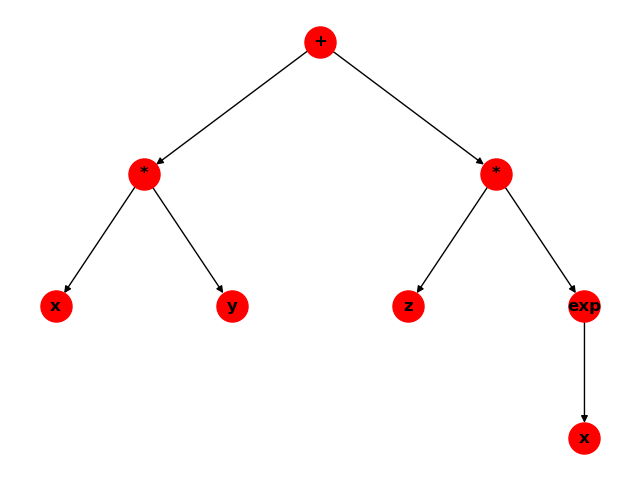
\includegraphics{chapters/images/AST.png}
    \caption{Абстрактное синтаксическое дерево выражения $x \cdot y + z \cdot exp(x)$}
    \label{fig:AST}
\end{figure}

В нашем случае мы получаем на вход строковое представление математического выражения, а возвращаем дерево разбора, состоящее из внутренних узлов, представляющий математические функции, например как сложение или взятие логарифма, и листьев, состоящих из переменных и чисел.

Абстрактное синтаксическое дерево (\textit{АСД}, \textit{AST}) отличается от дерева разбора тем, что в нём отсутствуют узла и рёбра, которые не влияют на семантические свойств выражения. Например, для выражения $3 + 2 \cdot 4$ не нужно расставлять группирующие скобки, так как приоритет операции умножения задан выше, чем приоритет операции сложения.

Многие языки программирования и системы компьютерной алгебры используют данный подход для обработки для обработки своих выражений. В частности, АСД использует фреймворк SymPy \cite{SymPy}, реализованный на языках программирования Python и Julia, который мы будем использовать в дальнейшем.

Подробнее ознакомиться с синтаксическими деревьями можно в \cite{Automata-book}, \cite{Compilers-book}

\subsection{Алгоритм полиномиализации} \label{poly-algo}

Для начала перепишем алгоритмы из секций \ref{sec:poly-algebraic}, \ref{sec:poly-diff} в формальном общем виде. Как уже упоминалось в разделе \ref{sec:AST}, нам удобно представлять правые части уравнений системы в виде абстрактных синтаксических деревьев. Из таких деревьев мы формируем лес, которые впоследствии мы будем анализировать.

\begin{algorithm}[H]
\SetAlgoLined
\SetKwFunction{FPoly}{Polynomialize}
\SetKwFunction{FGetNonPoly}{GetNonPolynomialItem}
\SetKwFunction{FFindNonPoly}{FindNonPolynomialItem}
\SetKwProg{Fn}{Function}{:}{}
\KwData{System - система вида \eqref{eq:ODE-norm-system} или \eqref{eq:ADE-system}}
\KwResult{Полиномиализированная система}
\Fn{\FPoly{System}}{
    NewSystem = Копия(System)\;
    
    \tcc{Лес абстрактных синтаксических деревьев}
    Forest = \{\quad\}\;
    
    \tcc{массив меток, где true - данное дерево не содержит неполиномиальных элементов}
    ForestIsPoly = \{\quad\}\;
    
    \ForEach{r: правое уравнение системы}{
        tree = AST(r)\;
        Добавить(Forest, tree)\;
        ForestIsPoly[tree] = false\;
    }
    
    \While{ForestIsPoly содержит false}{
        g = \FGetNonPoly{Forest, ForestIsPoly}\;
        ДобавитьУравнение(NewSystem, g)\;
    }
    
    \Return NewSystem\;
}
\BlankLine
\BlankLine
\Fn{\FGetNonPoly{Forest, ForestIsPoly}}{
    \ForEach{tree: ForestIsPoly[tree] == false}{
        nonPolyItem = \FFindNonPoly{tree}\;
        \eIf{nonPolyItem $\ne$ null }{
            \Return nonPolyItem\;
        }{
            ForestIsPoly[tree] = true\;
        }
    }
    \Return null\;
}
\caption{Полиномиализация}
\end{algorithm}

\subsubsection{Прямой обход}

Разберём вариант реализации алгоритма FindNonPolynomialItem, который предполагает прямой проход по синтаксическому дереву - от корня к листьям. \\

\begin{algorithm}[H]
\SetAlgoLined
\SetKwFunction{FFindNonPoly}{FindNonPolynomialItem}
\SetKwProg{Fn}{Function}{:}{}
\KwData{node - узел AST, составленного из правой части уравнения системы \eqref{eq:ODE-norm-system} или \eqref{eq:ADE-system}}
\KwResult{Неполиномиальный элемент или null, если такой не найдётся}

\Fn{\FFindNonPoly{node}}{
    \If{неПолиномиальнаяФункция(node)}{
        \Return node\;
    }
    
    \ForEach{child: дети node}{
        nonPolyItem = \FFindNonPoly{child}\;
        \If{nonPolyItem $\ne$ null}{
            \Return nonPolyItem\;
        }
    }
    \Return null\;
}

\caption{Прямой обход синтаксического дерева}
\end{algorithm}

\newpage

\subsubsection{Обратный обход}

Теперь рассмотрим вариант реализации алгоритма FindNonPolynomialItem, который предполагает обратный проход по синтаксическому дереву - от листьев к корню. \\

\begin{algorithm}[H]
\SetAlgoLined
\SetKwFunction{FFindNonPoly}{FindNonPolynomialItem}
\SetKwProg{Fn}{Function}{:}{}
\KwData{node - узел AST, составленного из правой части уравнения системы \eqref{eq:ODE-norm-system} или \eqref{eq:ADE-system}}
\KwResult{Неполиномиальный элемент или null, если такой не найдётся}

\Fn{\FFindNonPoly{node}}{
    \ForEach{child: дети node}{
        nonPolyItem = \FFindNonPoly{child}\;
        \If{nonPolyItem $\ne$ null}{
            \Return nonPolyItem\;
        }
    }
    
    \If{неПолиномиальнаяФункция(node)}{
        \Return node\;
    }
    \Return null\;
}

\caption{Обратный обход синтаксического дерева}
\end{algorithm}

\subsubsection{Сравнение}

Прямой и обратный обходы по синтаксическому дереву похожи на поиск в ширину и поиск в глубину соответственно. \\

Прямой обход последовательно проходит уровни глубины синтаксического дерева, возвращая первый встреченный неполиномиальный элемент. Таким образом, данный алгоритм работает быстрее, чем обратный подход в том случае, когда  нелинейный элемент находится неглубоко, что характерно для для практических задач. Однако важно помнить, что если найденный нелинейный элемент является композицией функций $g = g_1 \circ g_2 \circ \cdots \circ g_k$, то прямой обход вернёт всю композицию. Это является существенным недостатком, если мы используем алгоритм \ref{sec:poly-diff}, требующий вычислять сложную производную функции $g$, что является весьма дорогой операцией для композиции функций.

Обратный обход, в свою очередь, ищет самые глубоко вложенные неполиномиальные элементы $g_k$. Поэтому, он всегда находит базовые элементарные функции, имеющие тривиальные производные, затрачивая, в целом, большее число шагов.    

\begin{example}
    Для выражения $x + \sin{(\exp{x})}$ прямой обход найдёт найдёт $\sin{(\exp{x})}$, а обратный - $\exp{x}$.
\end{example}

Таким образом, для полиномиализации \ref{sec:poly-algebraic} мы предпочтём прямой обход, а для \ref{sec:poly-diff} - обратный.

% !TEX root = ../Диплом.tex

\section{Квадратизация} \label{sec:quadratiaztion}

\begin{definition}
    Процесс преобразования нелинейных систем \ref{eq:ODE-norm-system}, \ref{eq:ADE-system} к квадратичному виду будем называть \textit{квадратизацией}.
\end{definition}

В данном разделе мы будем рассматривать оригинальные алгоритмы квадратизации, применимые только для  полиномиальных систем \cite{Gu-PhD}. Мы уже описали способы получения таких систем из систем \ref{eq:ODE-norm-system}, \ref{eq:ADE-system} в секции \ref{sec:polynomialization}. Так же заметим, что подходы, применяемые для квадратизации систем, весьма похожи на методы полиномиализации.

\subsection{Квадратизация с помощью введения алгебраических уравнений} \label{sec:quad-algebraic}

Данный алгоритм квадратизует систему, добавляя к ней алгебраические уравнения.

\begin{enumerate}
    \item Ввести новую переменную $y_i = m_i(\vec x)$, где $m_i(\vec x) = x_1^{b_1}\cdot \cdots \cdot x_n^{b_n}$ - моном, образованный из переменных системы.
    \item Заменить $m_i(\vec x)$ на $y_i$ в оригинальном уравнении.
    \item Добавить новое уравнение $y_i = m_i(\vec x)$ в систему.
\end{enumerate}

Показанный алгоритм приводит полиномиальные системы вида \eqref{eq:ODE-norm-system}, \eqref{eq:ADE-system} к квадратичным системам вида \eqref{eq:ADE-system}.

\begin{example}
    Квадратизуем систему, полученную в примере раздела \ref{sec:poly-algebraic}:

    $\begin{array}{lcl}
        \dot x = x^3 + y_1 \\
        0 = xy_1 + y_1 - 1
    \end{array}$
    \newline
    
    Теперь проведём квадратизацию:
    
    \begin{enumerate}
    	\item Вводим новую переменную $y_2 =  x^2$
    	\item Делаем замену в первом уравнении $\dot x = xy_2 + y_1$
    	\item Добавляем новое уравнение в систему $y_2 - x^2 = 0$
    \end{enumerate}
    
    Получили квадратичную систему
    
    $\begin{array}{lcl}
        \dot x = xy_2 + y_1 \\
        0 = xy_1 + y_1 - 1 \\
        0 = y_2 - x^2
    \end{array}$
\end{example}


\subsection{Квадратизация с помощью введения дифференциальных уравнений} \label{sec:quad-diff}

Следующий алгоритм проводит квадратизацию, добавляя в систему ОДУ:

\begin{enumerate}
    \item Ввести новую переменную $y_i = m_i(\vec x)$, где $m_i(\vec x) = x_1^{b_1}\cdot \cdots \cdot x_n^{b_n}$ - моном, образованный из переменных системы.
    \item Заменить $m_i(\vec x)$ на $y_i$ в оригинальном уравнении
    \item Добавить новое уравнение $\dot y_i = \dot {m_i}(\vec x) = m'_i(\vec x) \dot{\vec x}$ в систему, где $m'(\vec x) = \frac {dm(\vec x)}{d \vec x}$
\end{enumerate}

Данный алгоритм переводит полиномиальные системы к квадратичному виду, не меняя их структуры: \eqref{eq:ODE-norm-system} $\longrightarrow$ \eqref{eq:ODE-norm-system}, \eqref{eq:ADE-system} $\longrightarrow$ \eqref{eq:ADE-system}.

\begin{example}
    Рассмотрим систему

    $\begin{array}{lcl}
        \dot x = xz^2 + z \\
        \dot z = x \\
    \end{array}$
    \newline
    
    Теперь проведём квадратизацию:
    \begin{enumerate}
        \item Вводим новую переменную $y = z^2$
        \item Делаем замену в первом уравнении $\dot x = xy + z$
        \item Добавляем новое уравнение в систему $\dot y = 2z \dot z = 2xz$
    \end{enumerate}
    
     Получили квадратичную систему
    
    $\begin{array}{lcl}
        \dot x = xy + z \\
        \dot y = 2xz \\
        \dot z = x \\
    \end{array}$
\end{example}

\subsection{Анализ алгоритмов квадратизации} \label{sec:quad-analysis}

В отличии от полиномиализации, число введённых алгоритмами квадратизации \ref{sec:quad-algebraic}, \ref{sec:quad-diff} уравнений уже не является линейным относительно возможных замен переменных. Более того, как мы покажем далее, число возможных замен так же заметно больше. Поэтому нам становится важен вопрос об оптимальной по числу введённых уравнений квадратизации. Для этого нам понадобится использовать более продвинутые методы анализа, нежели чем для полиномиализации.

Так же заметим, что мы пользуемся только мономиальными заменами, что, вообще говоря, не даёт нам возможности получить оптимальную квадратизацию в общем случае, так как она может достигаться полиномиальными заменами.



\pagebreak

\subsection{Генерация замен переменных} \label{sec:replacement-generation}

Генерировать возможные мономиальные замены переменных из монома мы будем рекурсивно, постепенно деля изначальный моном, а далее мономы из его разложений на все их релевантные делители.

\begin{algorithm}[H]
\SetAlgoLined
\SetKwFunction{FGenRepl}{GenerateReplacements}
\SetKwFunction{FGenReplRec}{GenerateReplacementsRecursive}
\SetKwFunction{FUnique}{Уникальные}
\SetKwFunction{FAdd}{Добавить}
\SetKwFunction{FGenDivs}{СгенерироватьДелители}
\SetKwProg{Fn}{Function}{:}{}
\SetKwData{AllDec}{AllDecompositions}
\SetKwData{monomial}{monomial}
\SetKwData{dec}{decomposition}
\SetKwData{div}{делитель}
\SetKwData{divs}{делители}
\KwData{monomial - входной моном, чьи разложения мы хотим получить.}
\KwResult{Все релевантные разложения монома.}

\Fn{\FGenRepl{\monomial}}{
    \tcc{Множество всех разложений monomial}
    \AllDec = \{\quad\}\;
    \FGenReplRec{\monomial, \{\}, \AllDec}\;
    \Return \FUnique{\AllDec}\;
}
\BlankLine
\BlankLine
\Fn{\FGenReplRec{\monomial, \dec, \AllDec}}{
    \If{\dec не пусто}{
        \FAdd{\AllDec, \dec}\;
    }
    
    \tcc{Генерирует все делители монома степенью не менее 2 и не более $M$ - 1, где $M$ - степень \monomial}
    \divs = \FGenDivs{\monomial}\;
    
    \ForEach{\div: \divs}{
        \FGenReplRec{\monomial / \div, \FAdd{\dec, \div}, \AllDec}\;
    }
    
}
\caption{генерация замен переменных} \label{algo:Replacement-Gen}
\end{algorithm}

Таким образом, повторив эту процедуру для каждого уникального монома в полиномной системе, мы получим все возможные для неё замены переменных. 

\begin{example}
    $x^2y^3 \Longrightarrow (x, xy^3), (xy, xy^2), (x^2 y^3), (y, x^2 y^2)$ \linebreak $(y, x^2, y^2), (x, xy, y^2), (y^2, x^2 y), (y, xy, xy)$
\end{example}

Заметим, что приведённый алгоритм иллюстрирует лишь идеею получения замен и не является оптимальным способом это делать, так как алгоритм генерирует много эквивалентных разложений, представляющие собой одно и то же разложение, записанное в разном порядке.
\begin{example}
    $(x^2, xy, y^2) \sim (x^2, y^2, xy) \sim (xy, y^2, x^2) \sim \cdots$
\end{example}

Число таких перестановок $P_n - n!$, где $n$ - степень монома. Таким образом, сокращение числа перестановок, которые генерируются алгоритмом \ref{algo:Replacement-Gen}, можно считать главной задачей для его оптимизации. Мы предлагаем в качестве отправной точки попробовать создать дерево, основанное на сжатых префиксных и суффиксных деревьях. Так же, важно заметить, что моном фиксированной степени и числа переменных имеет единственный набор уникальных разложений. Поэтому, можно заранее вычислить все разложения для мономов, часто встречающихся на практике, и использовать их, не вычисляя в момент исполнения программы.

\subsection{Граф замен} \label{sec:replacement-graph}

Теперь обобщим процесс выбора замен переменных.

\begin{definition}
    \textit{Граф замен} - ациклический ориентированный граф, чьи вершины представляют системы уравнений, эквивалентные заданной системе, а дуги - преобразования, совершаемые с помощью замены переменной. Входной вершиной мы полагаем заданную систему, а выходной - систему, обладающей нужными нам свойствами.
\end{definition}


\begin{wrapfigure}[12]{l}[10pt]{9cm}
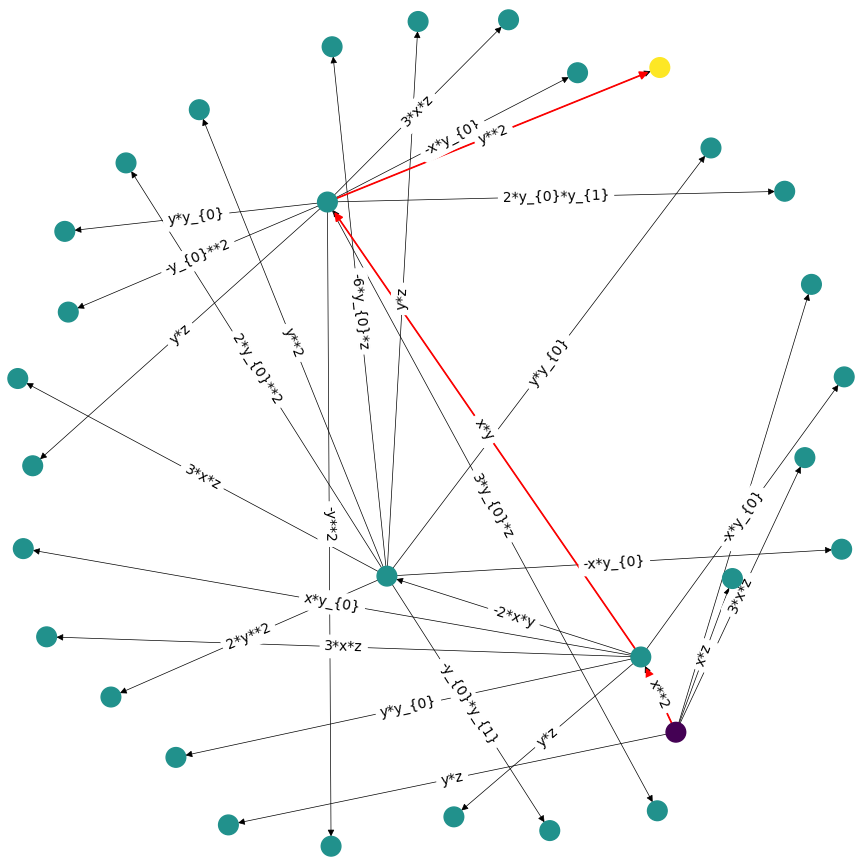
\includegraphics[width=9cm,height=9cm]{chapters/images/replacement_graph.png} 
\caption{Граф замен}
\label{fig:replacement-graph}
\end{wrapfigure}

Таким образом, мы можем трактовать задачу об оптимальной квадратизации как задачу поиска на графе с одним входом и несколькими выходами. Важно заметить, что графы замен, которые нам будут встречаться на практике, часто являются огромными и заранее задан только начальный узел, что делает неприменимыми значительную часть классических алгоритмов поиска.

\subsection{Алгоритмы поиска на графе} \label{sec:search-algo}

В данном разделе мы рассмотрим основные алгоритмы поиска на графе. Подчеркнём, что сам путь нас не интересует, поэтому мы приводим алгоритмы поиска пути на графах, которые, в связи с этим упрощаются.

Пусть $G$ - ориентированный граф, $V$ - множество его рёбер, $E$ - множество его дуг, $b$ - средний коэффициент ветвления $G$, $l$ - минимальная глубина выходного узла.

\subsubsection{BFS и DFS} \label{sec:BFS-DFS}

Поиск в глубину (depth-frist search, DFS) и поиск в ширину (breadth-first search BFS) являются базовыми в задаче поиска, нередко оказываясь достаточно эффективными для многих задач. К сожалению, в чистом виде применить данные алгоритмы для нашей задачи не представляется возможным. Действительно, глубина всего графа замен может быть близка к бесконечной при неаккуратном выборе замен, что критично для DFS. В случае BFS нам мешает высокий коэффициент ветвления, который, более того, растёт при для каждого последующего уровня глубины. Таким образом, BFS пригоден для практического использования только в том случае, когда искомая система находится на небольшой глубине. 

\subsubsection{Поиск с ограничением глубины (DLS)} \label{sec:DLS}

\begin{definition}
    \textit{Поиск с ограничением глубины} (depth-limited search, DLS) - вариант поиска в глубину, для которого определяется конечная глубина $l$ на которую он может опуститься. Таким образом, алгоритм всегда работает конечное число шагов, в отличие от DFS, однако ответ не может быть найден, если глубина выходного узла $d > l$.
\end{definition}

\begin{algorithm}[H]
\SetAlgoLined
\SetKwFunction{FDLS}{DLS}
\SetKwProg{Fn}{Function}{:}{}
\KwData{G - входной граф \\
    prop - свойство, которым должна обладать выходная вершина \\
    visited - массив, хранящий для каждой вершины бит, показывающий, посещали ли мы эту вершину \\
    l - предельная глубина}
\KwResult{Вершина, обладающая свойством prop или null, если вершина не найдена}

\Fn{\FDLS{G, v, prop, depth, l}}{
    visited[v] = true\;
    \If{v обладает свойством prop}{
        \Return v\;
    }
    \ForEach{w: сосед v}{
        \If{visited[w] == false \& depth < l}{
            \Return \FDFS(G, w, prop, depth + 1, l)\;
        }
    }
    \Return null\;
}
\caption{Поиск с ограничением глубины}  \label{algo:DLS}
\end{algorithm}

Данный алгоритм не уходит дальше заданной глубины, что решает проблему DFS и просматривает узлы на желаемой глубине, а не последовательно идя по слоям, как BFS. Таким образом, при удачно выбранной конечной глубине и хорошем выборе замен на каждом шаге, мы сможем решать задачу за сравнительно небольшое число шагов.

Однако, если мы оценили конечную глубину ниже, чем глубину искомой вершины, то решить задачу мы не сможем. Решает эту проблему следующий алгоритм поиска. 

\subsubsection{Поиск в глубину с итеративным углублением (ID-DFS)} \label{sec:ID-DFS}

\begin{definition}
    \textit{Поиск в глубину с итеративным углублением} (iterative-deepening depth-first search, ID-DFS) запускает DLS на каждой своей итерации и, в случае неудачи, увеличивает конечную глубину $l$.
\end{definition}

\begin{algorithm}[H]
\SetAlgoLined
\SetKwFunction{FIDDFS}{IDDFS}
\SetKwFunction{FDLS}{DLS}
\SetKwProg{Fn}{Function}{:}{}
\SetKwRepeat{Do}{do}{while}
\KwData{G - входной граф \\
prop - свойство, которым должна обладать выходная вершина}
\KwResult{Вершина, обладающая свойством prop или null, если вершина не найдена}

 \Fn{\FIDDFS{G, v_{start}, prop}}{
    l = 1\;
    
    \Do{v == null}{
        v = \FDLS{G, v, prop, 1, l}\;
        l += 1\;
    }
    \Return v\;
 }
\caption{Поиск в глубину с итеративным углублением} \label{algo:ID-DFS}
\end{algorithm}

Не смотря на то, что ID-DFS гарантирует нахождение выходной вершины, в отличие от DLS, у него есть 2  существенных недостатка:
\begin{enumerate}
    \item Необходимость исследовать граф заново, если на текущей итерации выходную вершину найти не получилось.
    \item Увеличение глубины происходит всегда на 1, что не всегда является оптимальной стратегией.
\end{enumerate}

Поэтому мы несколько модифицируем ID-DFS, чтобы устранить данные недостатки.

\subsubsection{Поиск с ограничением глубины и итеративным углублением (ID-DLS)} \label{sec:ID-DLS}

\begin{definition}
   Введём новый алгоритм \textit{Поиск с ограничением глубины с итеративным углублением} (\textit{ID-DLS}), который отличается от ID-DFS в следующем:

    \begin{enumerate}
        \item Вместо исследования графа заново после неудачной итерации, ID-DLS сохраняет вершины на текущей конечной глубине вместе с их исходящими заменами. В случае неудачного поиска мы сразу начинаем вычислять неисследованные элементы. Платой за это становится удвоенные затраты на память.
        \item Текущая конечная глубина более гибко изменяется за счёт функции $ОбновитьТекущуюКонечнуюГлубину$. Платой за это становится то, что гарантия оптимальности квадратизации ложится на приведённую функцию. Тем не менее, таким образом мы может искать суб-оптимальные решения с погрешностью, также определяемой функцией $ОбновитьТекущуюКонечнуюГлубину$.
    \end{enumerate} 
\end{definition}


\begin{algorithm}[H]
\SetAlgoLined
\SetKwFunction{FIDDLS}{IDDLS}
\SetKwFunction{FDLS}{DLS}
\SetKwProg{Fn}{Function}{:}{}
\SetKwRepeat{Do}{do}{while}
\KwData{G - входной граф \\
$v_{start}$ - входная вершина \\
prop - свойство, которым должна обладать выходная вершина \\
limit - финальная конечная глубина}
\KwResult{Вершина, обладающая свойством prop или null, если вершина не найдена}

 \Fn{\FIDDLS{G, v_{start}, prop, limit}}{
    currentLimit = 1\;
    
    \tcc{В данную очередь помещаются элементы на текущей конечной глубине вместе с их исходящими заменами. Фактически, мы лениво вычисляем вершины со следующего уровня}
    highDepthQueue = \{\ \}\;
    
    \Do{v == null}{
        \If{currentLimit > limit}{
            \Return null
        }
        v = \FDLS{G, v, prop, 1, currentLimit, highDepthQueue}\;
        currentLimit = ОбновитьТекущуюКонечнуюГлубину(currentLimit)\;
    }
    \Return v\;
 }
\caption{Поиск с ограничением глубины с итеративным углублением} \label{algo:ID-DLS}
\end{algorithm}

Дополнительным улучшением к данному алгоритму могут послужить эффективные оценки верхней и нижней границ минимальной глубины выходного узла $l$, которые позволят просматривать как можно меньше неперспективных узлов.

\subsection{Эвристический подход к поиску} \label{sec:heuristics-intro}

Эвристический поиск, он же информированный поиск представляет собой семейство стратегий поиска,
в котором используются знания о конкретной задаче, зачастую позволяя решать задачу поиска гораздо эффективнее.

Знания о задаче формализуются в качестве эвристических функций.
Эвристические функции сравнивают между собой варианты, из которых алгоритм выбирает следующий шаг.

В случае задач поиска на графе, с помощью эвристических функций мы будем сортировать дуги алгоритмов неинформированного поиска.

Приведём эвристические версии алгоритмов неинформированного поиска
\begin{enumerate}
    \item DFS $\rightarrow$ Поиск по первому наилучшему совпадению (best-first search)
    \item Алгоритм Дейкстры $\rightarrow$ Алгоритм A*
    \item ID-DFS $\rightarrow$ Алгоритм А* с итеративным углублением (Iterative deepening A*, IDA*)
\end{enumerate}


\subsection{Эвристики для квадратизации} \label{sec:quad-heuristics}

Точкой ветвления алгоритма квадратизации является шаг, на котором мы выбираем, в какой порядке исследовать возможные замены переменных. Таким образом, определим семейство эвристических функций в задаче квадратизации как 

\begin{equation}
    h:\ \mathbb{M} \longrightarrow \mathbb{R},
\end{equation}
где $\mathbb{M}$ - группа мономов, образованных над переменными $\vec x$ полиномных систем \eqref{eq:ODE-norm-system}, \eqref{eq:ADE-system}. 

\begin{heuristics} \label{heur:FF}
    \textit{Frequent-First}, \textit{FF} - эвристика, выбирающая моном, наиболее часто встречающийся в разложениях. Таким образом, замена переменной затронет наибольшее число мономов в системе.
    
    \begin{example}
        Для разложений $(x^2, xy), (xy, y^2, y^3, xy^2, xy^3), (x^2, y^2, xy)$ мы выберем моном $xy$, так как он встречается в трёх разложениях, а остальные не более чем в двух.
    \end{example}
\end{heuristics}

\begin{heuristics} \label{heur:FVC}
    \textit{Free-Variables-Count}, \textit{FVC} - эвристика, выбирающая моном, образованный из наименьшего числа    переменых. Таким образом, в уравнении $y_i = m'(\vec x) \dot{\vec x}$, соответствующем данной замене, будет минимальное число слагаемых.
    
    \begin{example}
        Из мономов $x^2, xy, xyz$ мы выберем $x^2$, имеющий только одну переменную. Покажем ОДУ, образованные данными заменами:
        \begin{enumerate}
            \item $x^2 \longrightarrow \dot w = 2x \dot x$
            \item $xy \longrightarrow \dot w = \dot x y + x \dot y$
            \item $xyz \longrightarrow \dot w = \dot x yz + x \dot y z + xy \dot x$
        \end{enumerate}
    \end{example}
\end{heuristics}

\begin{heuristics} \label{heur:AED}
    \textit{Auxiliary-Equation-Degree}, \textit{AED} - эвристика, выбирающая моном, порождающий уравнение с наименьшей степенью. 
    
    \begin{example}
        Пусть имеем систему со следующим респределение степеней: $degree(\dot x) = 1,\ degree(\dot y) = 2$. Тогда для замен $x^2, xy, y^2$ получим степени уравнений:
        \begin{enumerate}
            \item $x^2 \longrightarrow \dot w = 2x \dot x \longrightarrow 1 + 1 = 2$
            \item $xy \longrightarrow \dot w = \dot x y + x \dot y \longrightarrow max(1 + 1, 1 + 2) = 3$
            \item $y^2 \longrightarrow \dot w = 2y \dot y \longrightarrow 1 + 2 = 3$
        \end{enumerate}
        Из данных замен выберем $x^2$.
    \end{example}
\end{heuristics}

\begin{heuristics} \label{heur:AEQD}
    \textit{Auxiliary-Equation-Quadratic-Discrepancy}, \textit{AEQD} - эвристика, выбирающая моном, чьё порождённое уравнение наименее отличается от квадратичного. Таким образом, замены, порождающие кважратичные уравнения, имеют самый высокий приоритет. 
    
    \begin{example}
        Пусть имеем замены, порождающие следующие уравнения
        \begin{enumerate}
            \item $m_1 \longrightarrow \dot w = x + y^2 + z^3 \longrightarrow 0 + 0 + 1 = 1$
            \item $m_2 \longrightarrow \dot w = x + y^2 + xy + z^3 \longrightarrow 0 + 0 + 0 + 1 = 1$
            \item $m_3 \longrightarrow \dot w = x + y^2 + z^3 + xyz \longrightarrow 0 + 0 +1 + 1 = 2$
        \end{enumerate}
        Таким образом, $m_1$ и $m_2$ имеют одинаковый приоритет, потому что порождённые ими уравнений имеют минимальную степерь 1.
    \end{example}
\end{heuristics}

\begin{heuristics} \label{heur:AEQD}
    \textit{Summary-Monomial-Degree}, \textit{SMD} - эвристика, представляющая развитие идеи FF. Мы вибираем замену, которая максимально понижает степерь системы.
    
    \begin{example}
        Рассмотрим систему
        
        $\begin{array}{lcl}
             \dot x = xy^2 + y^3 \\
             \dot y = xy + x^2 y + 1
        \end{array}$
        \newline
        
        Понижение степени системы для замены $m$ вычисляетя как $N \cdot (degree(m) - 1)$, где $N$ - число мономов в системе, которые нацело делятся на $m$.
        \begin{enumerate}
            \item $y^2 \longrightarrow 2 \cdot (2 - 1) = 2$
            \item $xy \longrightarrow 3 \cdot (2 - 1) = 3$
            \item $y^3 \longrightarrow 1 \cdot (3 - 1) = 2$
        \end{enumerate}
        Получили, что замена $xy$ максимально сильно снижает степень системы.
    \end{example}
\end{heuristics}

\subsection{Правило параллелограмма} \label{sec:parallel-rule}

Пусть для начальной полиномиальной системы $S$ имеются две замены $m_1$ и $m_2$.

\begin{wrapfigure}{R}{0.8\textwidth}
\begin{subfigure}{.4\textwidth}
  \centering
  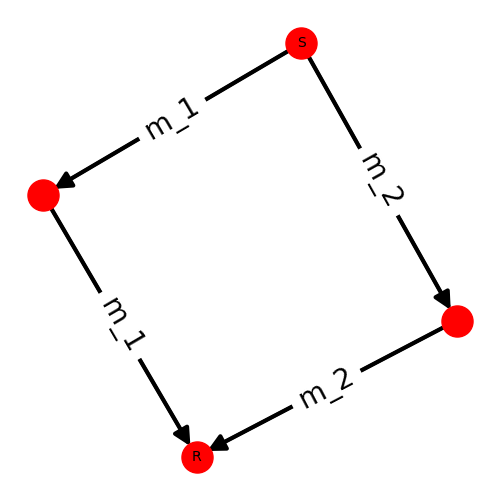
\includegraphics[width=0.8\linewidth]{chapters/images/parallel.png}  
  \caption{Граф замен для $S$}
  \label{fig:parallel-replacement-graph}
\end{subfigure}
\begin{subfigure}{.4\textwidth}
  \centering
  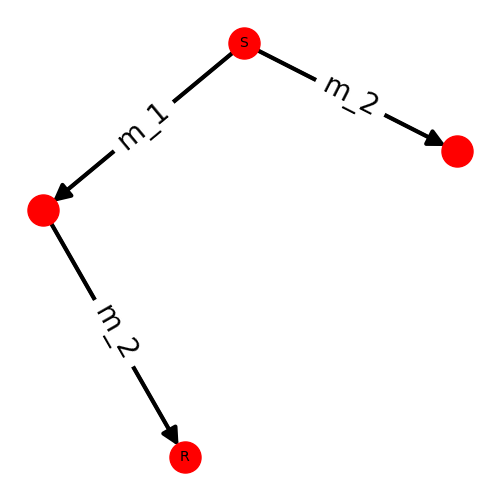
\includegraphics[width=0.8\linewidth]{chapters/images/parallel_red.png}  
  \caption{Упрощённый по правилу параллелограмма граф \ref{fig:parallel-replacement-graph}}
  \label{fig:parallel-replacement-graph-red}
\end{subfigure}
\caption{Правило параллелограмма}
\label{fig:parallel-rule}
\end{wrapfigure}

\begin{proposition}
    Замены $m_1$ и $m_2$ приведут к одной и той же системе $R$ вне зависимости от порядка их проведения. Действительно, ведь в таком случае введённые переменные $y_1$ и $y_2$ получаются перестановкой $[y_1 = y_2,\; y_2 = y_1]$.
\end{proposition}

Таким образом, мы можем убирать часть рёбер из графа во время его исследования. Данная оптимизация становится весьма важна для параллельных версий алгоритма, так как даёт возможность потокам оптимизировать работу друг друга.


\begin{thebibliography}{9}
\bibitem{Gu-PhD} Gu C. Model order reduction of nonlinear dynamical systems : дис. – UC Berkeley, 2011.
\bibitem{Kramer-Willcox} Kramer B., Willcox K. E. Nonlinear model order reduction via lifting transformations and proper orthogonal decomposition //AIAA Journal. – 2019. – Т. 57. – №. 6. – С. 2297-2307.
\bibitem{Harrington-vanGorder} Harrington H. A., Van Gorder R. A. Reduction of dimension for nonlinear dynamical systems //Nonlinear Dynamics. – 2017. – Т. 88. – №. 1. – С. 715-734.
\bibitem{ID-DFS} Korf R. E. Depth-first iterative-deepening: An optimal admissible tree search //Artificial intelligence. – 1985. – Т. 27. – №. 1. – С. 97-109.
\bibitem{physics-example} Blackmore D. L. et al. Nonlinear dynamical systems of mathematical physics: spectral and symplectic integrability analysis. – World Scientific, 2011.
\bibitem{chemistry-example} Karri R. R. Evaluating and estimating the complex dynamic phenomena in nonlinear chemical systems //International Journal of Chemical Reactor Engineering. – 2011. – Т. 9. – №. 1.
\bibitem{biology-example} Jackson T., Radunskaya A. (ed.). Applications of Dynamical Systems in Biology and Medicine. – Springer, 2015. – Т. 158.
\bibitem{economics-example} Lines M. (ed.). Nonlinear dynamical systems in economics. - Springer Science \& Business Media, 2007. - Т. 476.
\bibitem{MOR-book} Schilders W. H. A., Van der Vorst H. A., Rommes J. Model order reduction: theory, research aspects and applications. – Berlin : Springer, 2008. – Т. 13.
\bibitem{Strogatz-book} Strogatz S. H. Nonlinear dynamics and chaos with student solutions manual: With applications to physics, biology, chemistry, and engineering. – CRC press, 2018.
\bibitem{Scott-reachability} Shen K., Scott J. K. Rapid and accurate reachability analysis for nonlinear dynamic systems by exploiting model redundancy //Computers \& Chemical Engineering. – 2017. – Т. 106. – С. 596-608.
\bibitem{MOR-linear-overview} Antoulas A. C., Sorensen D. C. Approximation of large-scale dynamical systems: An overview. – 2001.
\bibitem{Automata-book} John E. Hopcroft, Rajeev Motwani, and Jeffrey D. Ullman. 2006. Introduction to Automata Theory, Languages, and Computation (3rd Edition). Addison-Wesley Longman Publishing Co., Inc., USA.
\bibitem{Compilers-book} Alfred V. Aho, Monica S. Lam, Ravi Sethi, and Jeffrey D. Ullman. 2006. Compilers: Principles, Techniques, and Tools (2nd Edition). Addison-Wesley Longman Publishing Co., Inc., USA.
\bibitem{SymPy} https://www.sympy.org/ru/index.html

\end{thebibliography}


\end{document} 